\documentclass[11pt,a4paper]{article}
\usepackage[utf8]{inputenc}
\usepackage[T1]{fontenc}
\usepackage[brazilian]{babel}
\usepackage{lmodern,graphicx,geometry,amsmath}
\geometry{margin=1.7cm}
\graphicspath{{prints/}}
\setlength{\parindent}{0pt}
\setlength{\parskip}{5pt}

\begin{document}
\begin{center}
\Large\textbf{Lista 7 -- O Problema da Seleção}
\end{center}

\section*{Questão 1 -- Mínimo e Máximo Simultâneos}
O algoritmo processa os elementos aos pares. Em cada par, compara os dois valores entre si e depois compara o menor com o mínimo atual e o maior com o máximo atual. São 3 comparações para cada 2 elementos.

Para $n$ ímpar, o primeiro elemento inicializa mínimo e máximo; os pares restantes usam $3\lfloor n/2\rfloor$ comparações. Para $n$ par, a primeira comparação escolhe mínimo e máximo iniciais, e as demais dão $1+3(n/2-1)=3n/2-2$. Nos dois casos, o limite pedido é respeitado. No exemplo com 10 valores, foram 13 comparações (o limite é 15). O tempo é $\Theta(n)$.

\begin{center}
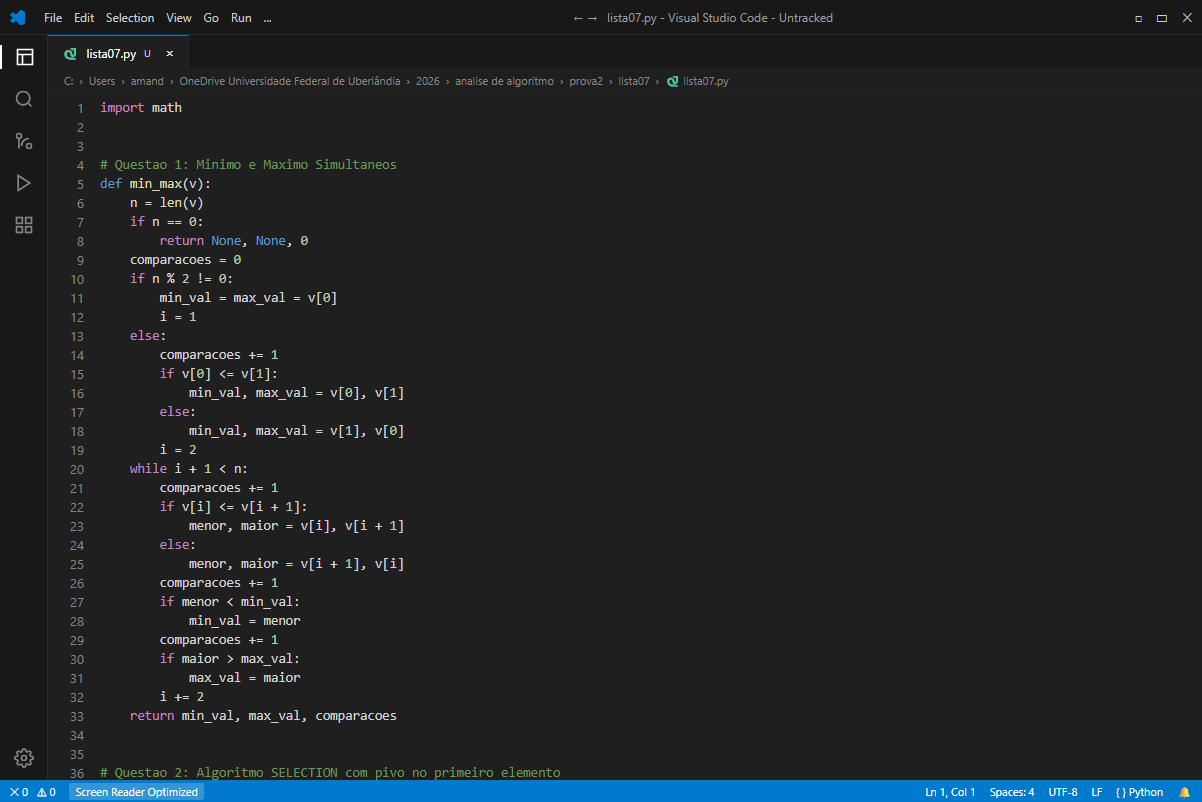
\includegraphics[width=15.6cm]{codigo_1.png}

\small Código aberto no VS Code.
\end{center}

\newpage
\section*{Questão 2 -- Algoritmo Selection}
Simulei o algoritmo de seleção para encontrar o 3º menor elemento ($i=3$) do vetor $\langle 1, 8, 7, 6, 5, 3, 2, 10, 9 \rangle$, mantendo o pivô fixo no primeiro elemento em cada partição.

Na primeira partição, o pivô é 1 na posição 1 ($k=1$); como todos os outros elementos são maiores, o pivô fica na posição 1. Como $i=3 > 1$, a busca segue recursivamente na sublista à direita $\langle 8, 7, 6, 5, 3, 2, 10, 9 \rangle$ com novo $i = 3 - 1 = 2$.
O novo pivô é 8, que ao particionar vai para a posição 7 ($k=6$ no subvetor). Como $i=2 \le 6$, a busca vai para o lado esquerdo $\langle 2, 7, 6, 5, 3 \rangle$ procurando o 2º menor. O pivô 2 fica na posição 2 ($k=1$), e como $i=2 > 1$, vamos à direita procurando o $2 - 1 = 1$º menor na lista $\langle 7, 6, 5, 3 \rangle$. O pivô 7 vai para o final ($k=4$), e buscando o 1º menor à esquerda encontramos o pivô 3 na posição final com $i=1=k$. O valor retornado é 3, exatamente o 3º menor elemento.

\begin{center}
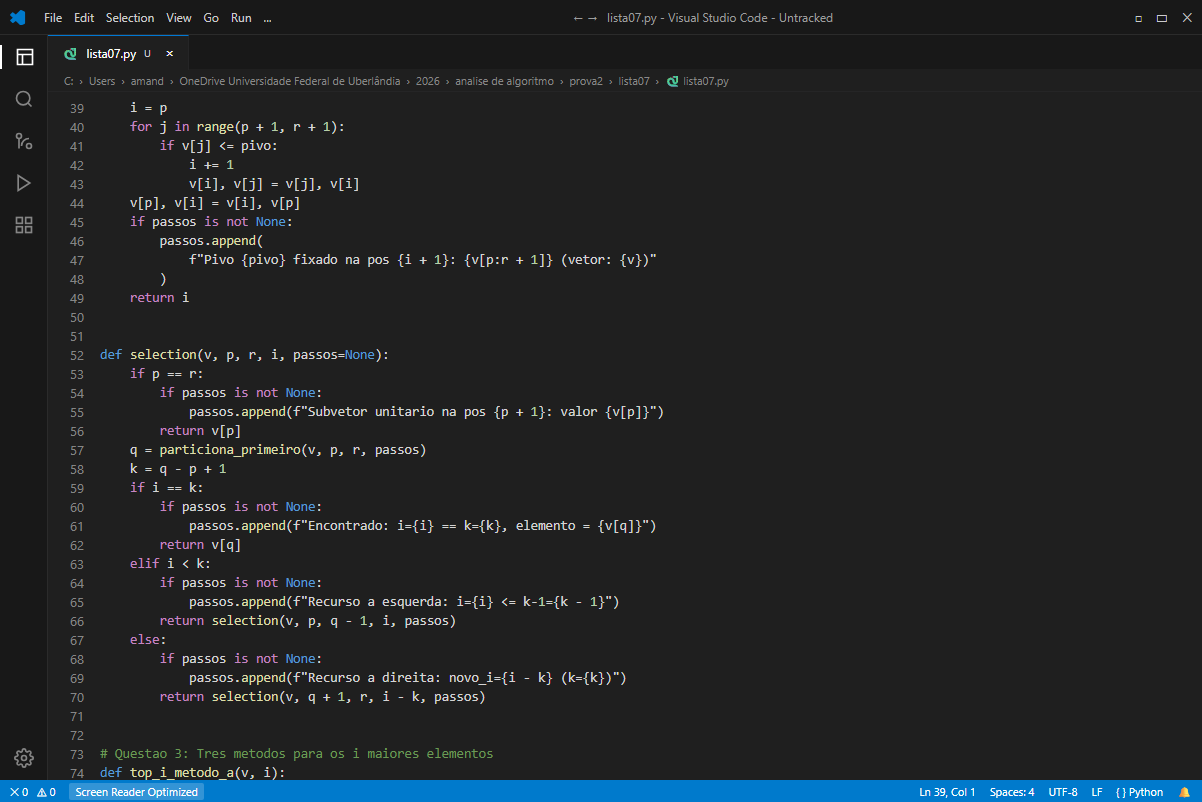
\includegraphics[width=15.6cm]{codigo_2.png}

\small Código da função Selection com pivô no primeiro elemento.
\end{center}

\newpage
\section*{Questão 3 -- Impressão dos $i$ Maiores Elementos}
Há três jeitos de obter os $i$ maiores elementos em ordem crescente:
\begin{itemize}
\item \textbf{Método A (Ordenação total):} ordena todo o vetor de tamanho $n$ (com MergeSort ou Heapsort) em tempo $\Theta(n\log n)$ e depois imprime os $i$ maiores em $\Theta(i)$, resultando em tempo total $\Theta(n\log n)$.
\item \textbf{Método B (Max-Heap):} constrói um max-heap com o vetor em tempo linear $\Theta(n)$ e realiza $i$ extrações de máximo com \texttt{HEAP-EXTRACT-MAX}, cada uma custando $\Theta(\log n)$. Invertendo a ordem das extrações para ficar crescente em $\Theta(i)$, o tempo total é $\Theta(n + i\log n)$.
\item \textbf{Método C (Seleção linear):} usa o algoritmo \texttt{SELECT} linear em tempo $\Theta(n)$ para encontrar o $(n-i+1)$-ésimo menor elemento (o corte dos $i$ maiores), particiona o vetor em torno dele em $\Theta(n)$ e ordena apenas o subvetor dos $i$ maiores em $\Theta(i\log i)$. O tempo total é $\Theta(n + i\log i)$.
\end{itemize}
Quando $i$ é pequeno, os métodos (b) e (c) podem evitar ordenar o vetor inteiro. O método (c) tem custo $\Theta(n+i\log i)$, enquanto o (b) tem custo $\Theta(n+i\log n)$; assim, o custo do (c) não é maior na análise assintótica.

No depurador, parei na primeira chamada do exercício 2. Dá para ver o pivô 1 e os limites do trecho que está sendo analisado.

\begin{center}
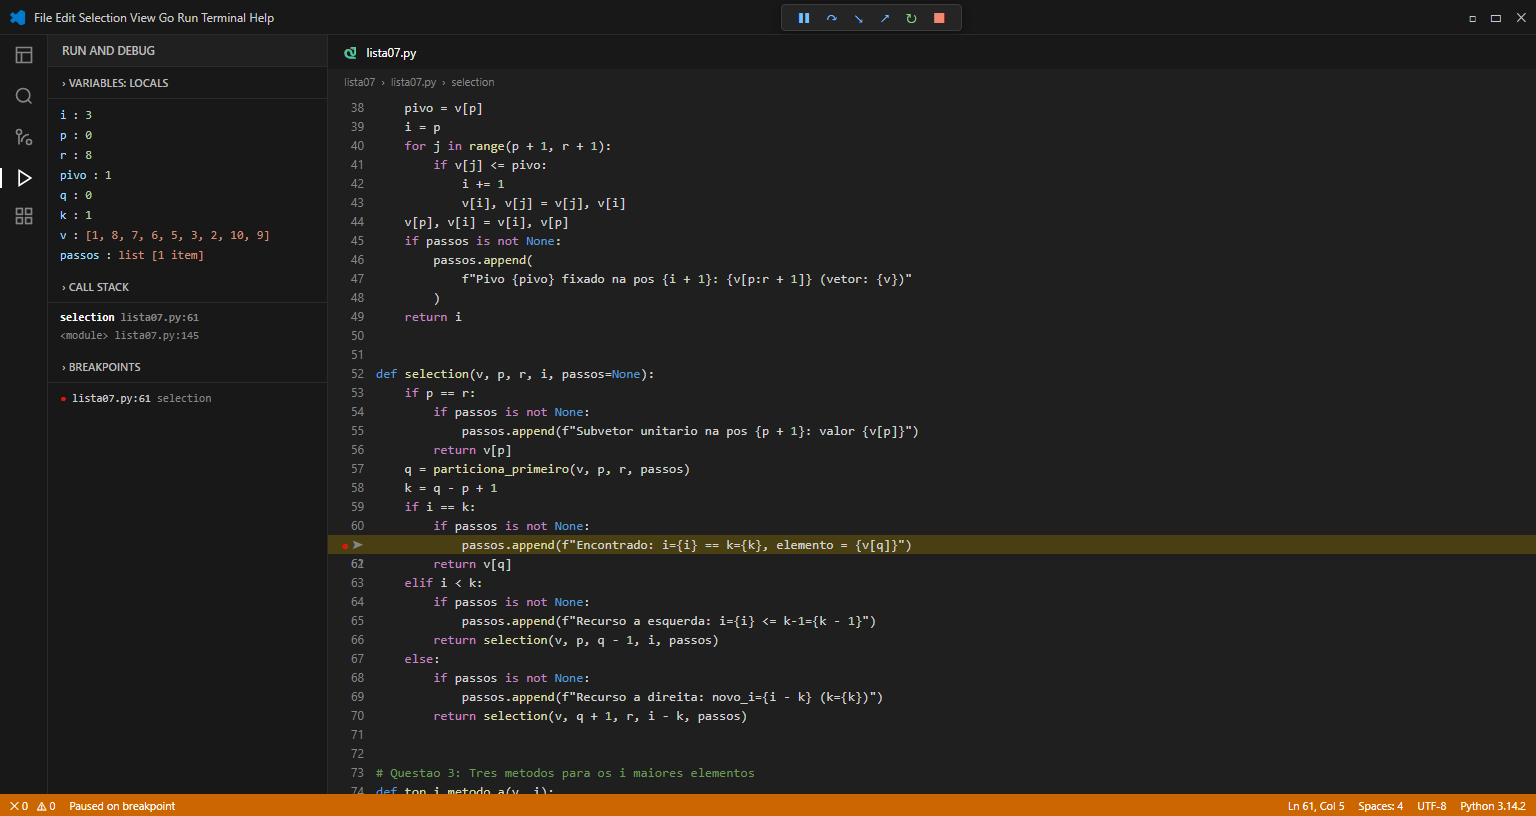
\includegraphics[width=15.6cm]{debug_exercicio.png}

\small Exercício 2 rodando no depurador do VS Code.
\end{center}

\newpage
\section*{Questão 4 -- QuickSort em Tempo $\Theta(n\log n)$ no Pior Caso}
O QuickSort pode levar $\Theta(n^2)$ quando as partições ficam muito desbalanceadas. Uma forma de evitar isso é escolher a mediana do trecho como pivô. Encontrá-la pelo algoritmo determinístico de seleção custa $\Theta(n)$.

Com esse pivô, os dois lados ficam com tamanho próximo de $n/2$. A recorrência é $T(n)=2T(n/2)+\Theta(n)$, que resulta em $\Theta(n\log n)$ no pior caso.

\begin{center}
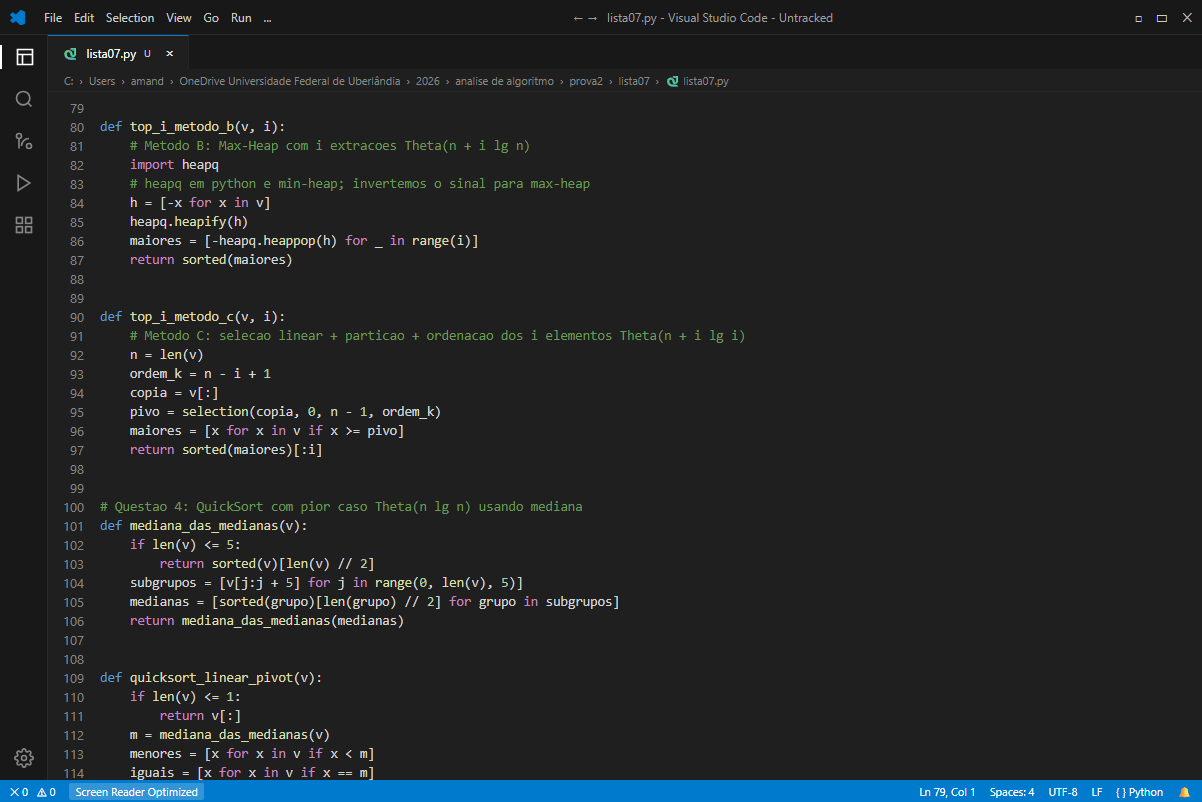
\includegraphics[width=12.8cm]{codigo_3.png}

\small Código dos métodos para os $i$ maiores e do QuickSort com mediana usado no programa.

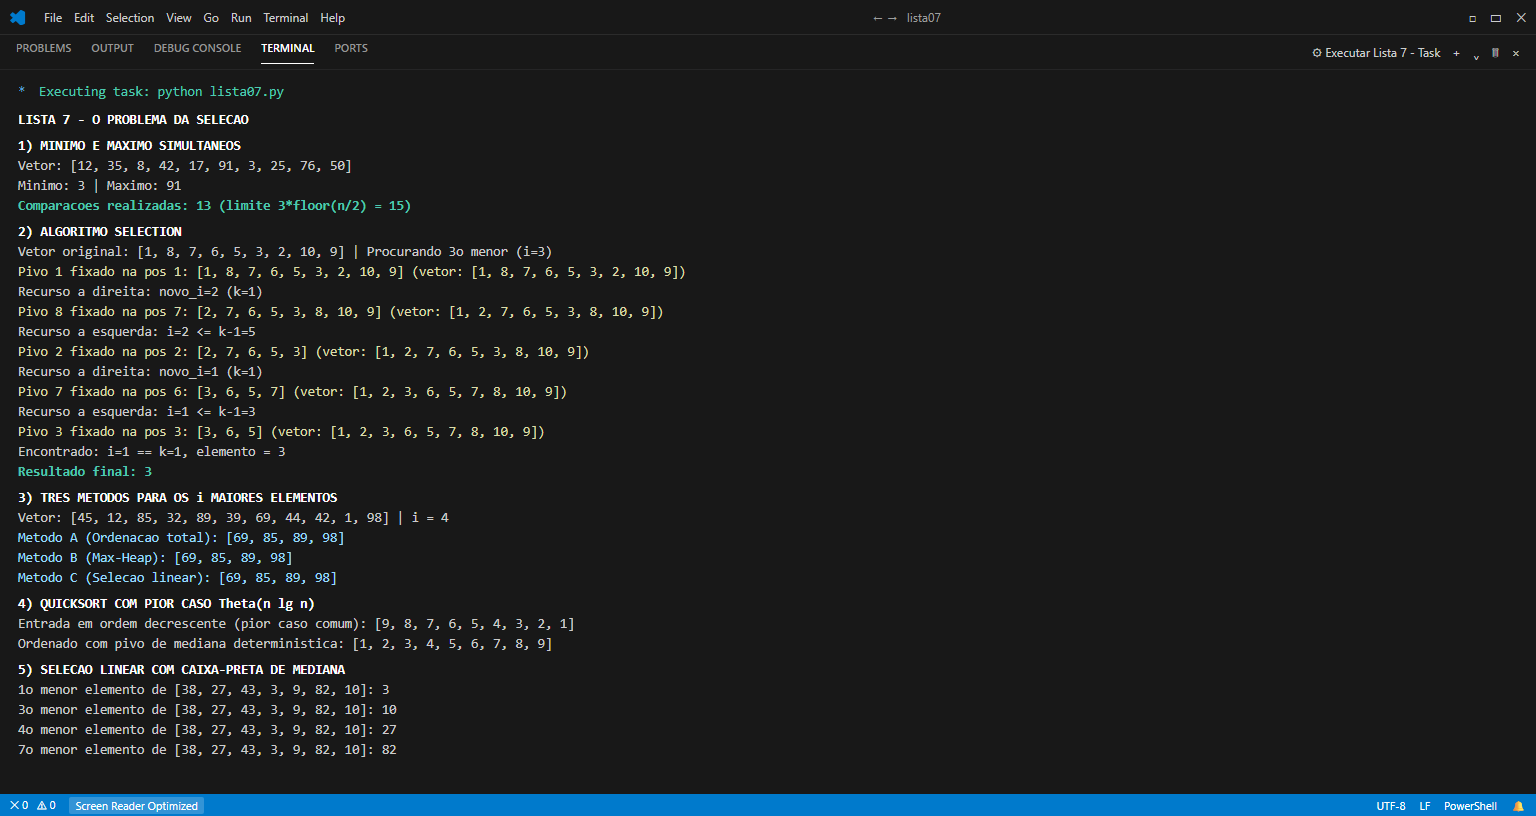
\includegraphics[width=13.8cm]{terminal_execucao.png}

\small Execução no terminal do VS Code. O comando \texttt{python lista07.py} aparece no início do terminal e o programa terminou mostrando os resultados.
\end{center}

\newpage
\section*{Questão 5 -- Seleção Linear com Caixa-Preta de Mediana}
Se existe uma rotina que encontra a mediana em tempo linear, podemos usá-la como pivô na seleção:
\begin{enumerate}
\item Chamo a caixa-preta para obter a mediana $m = \text{mediana}(A)$.
\item Particiono o vetor em três grupos: menores que $m$, iguais a $m$ e maiores que $m$, o que custa tempo linear $d\cdot n$. Como $m$ é a mediana exata, cada grupo tem no máximo $\lfloor n/2 \rfloor$ elementos.
\item Se $i \le |\text{menores}|$, busco recursivamente o $i$-ésimo menor em \texttt{menores}. Se $i$ estiver na faixa dos iguais, retorno $m$. Caso contrário, busco o $(i - |\text{menores}| - |\text{iguais}|)$-ésimo elemento em \texttt{maiores}.
\end{enumerate}
Em cada chamada, a recursão segue para apenas um lado, com no máximo metade dos elementos. A recorrência é $T(n)\le T(n/2)+cn$. Somando os custos $cn+cn/2+cn/4+\cdots$, obtemos tempo $\Theta(n)$ no pior caso.

\begin{center}
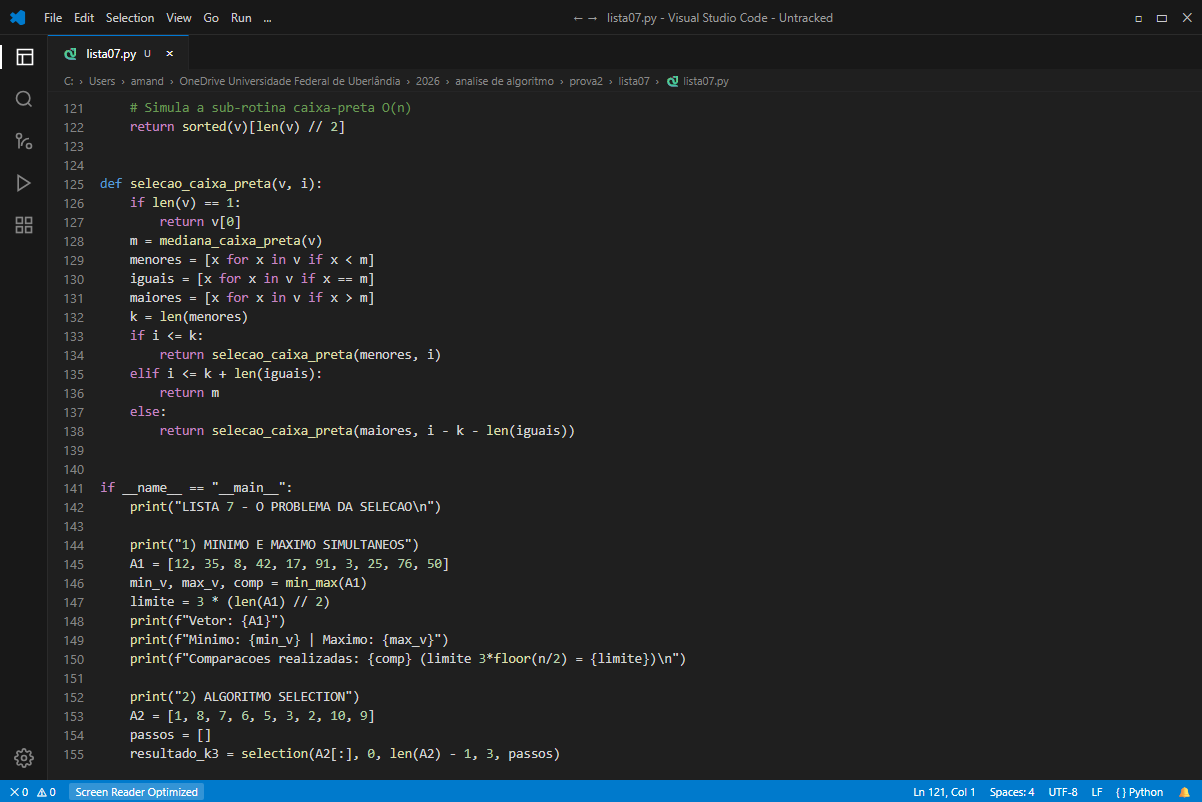
\includegraphics[width=15.6cm]{codigo_4.png}

\small Código da seleção linear com caixa-preta aberto no VS Code.
\end{center}

\end{document}
